\subsection{Elementos ferroviarios}

El sistema ferroviario consta de diversos elementos que incluyen la infraestructura (tendido ferroviario, plataformas, cruces de vía), sensores (circuitos de vía, contadores de eje), actuadores (barreras ferroviarias, máquinas de cambios) e interfaces visuales con los conductores (semáforos ferroviarios). Todos estos elementos se interrelacionan y funcionan en conjunto dentro del sistema de señalamiento y el sistema de enclavamiento. Cada uno de estos elementos será descripto en la sucesivas secciones, en orden tal de integrar los conceptos anteriores de la forma mas clara posible.

\subsubsection{Vías}

Las vías férreas son el elemento ferroviario mas esencial, son la columna vertebral de la infraestructura ferroviaria. Estas constituyen el sitio por el cual se desplazan los trenes, definiendo no solo la dirección del desplazamiento, sino también restringiendo el dominio del tren. Esto lo diferencia de otros medios de transporte como el automóvil que no necesitan un camino para circular y, aún teniendo una carretera, puede moverse libremente por fuera de esta.

Las vías se encuentran separadas por una distancia fija que se mide desde sus caras internas, denominada trocha (Figura \ref{fig:vias_1}). Solamente las formaciones compatibles con ese parámetro de trocha pueden circular por el tendido ferroviario. El valor de la trocha puede variar entre las denominadas trocha angosta (600 a 1372 mm, estándar imperial británico) y trocha ancha (1520 a 3000 mm, estándar ruso, indio, ibérico, irlandés). Se estableció el valor intermedio de 1425 mm como valor de trocha internacional, usado ampliamente en Europa, Norteamérica y Oceanía.

    \begin{figure}[!h]
        \centering
        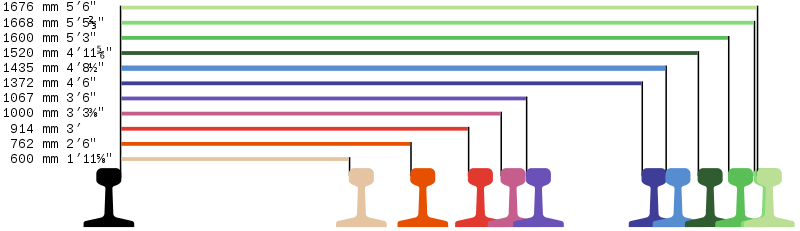
\includegraphics[width=1\textwidth]{Figuras/trocha.png}
        \centering\caption{Vías ferroviarias y trocha.}
        \label{fig:vias_1}
    \end{figure}
    
Existen limitaciones logísticas y físicas por las cuales el tendido ferroviario no puede ser un continuo rígido. En primer lugar, las vías deben ser de un tamaño acotado, tal que puedan transportarse a la locación donde serán instaladas en tramos rectos o curvos. En segundo lugar, la dilatación y contracción de las vías debido a los cambios de temperatura añaden una restricción respecto a la distancia mínima que deben tener entre las mismas. De lo contrario, la dilatación del material puede provocar daños irreparables a la infraestructura y estos, a su vez, ser motivo de descarrilamientos, como ya ha ocurrido en los comienzos de la industria ferroviaria [REF]. 
    
Cada vía puede ser clasificada en dos grupos: vías ascendentes o vías descendentes (\ref{fig:vias_2}). Las ascendentes son aquellas por las cuales los trenes circulan únicamente en la dirección del kilometraje en sentido creciente. Las descendentes son aquellas por las cuales los trenes circulan únicamente en la dirección del kilometraje en sentido decreciente [REF]. 

    \begin{figure}[!h]
        \centering
        \includegraphics[width=1\textwidth]{example-image}
        \centering\caption{Vías ascendentes y descendentes.}
        \label{fig:vias_2}
    \end{figure}

El kilómetro 0 es la estación principal de la línea ferroviaria, como pueden ser las terminales de Plaza Constitución (para la línea Roca), Once de septiembre (para la línea Sarmiento) y Retiro (para las líneas Mitre y San Martín).  Existen vías de maniobra que pueden ser tanto ascendentes como descendentes. Estas vinculan, mediante un cambio de vías, una sección ascendente con otra descendente, en la cual los trenes deben circular a una velocidad reducida. 

Las vías se agrupan en secciones que, por cuestiones de seguridad y logística, se establece que solo pueden ser utilizadas por un tren a la vez. Estas secciones pueden ser de varios kilómetros en zonas rurales o unos pocos cientos de metros en zonas urbanas, donde la red necesita una mayor granularidad debido a la densidad del tráfico ferroviario en las grandes urbes.
\subsubsection{Fin de vía y transiciones}

\lipsum[1]

\lipsum[1]
\includegraphics{example-image}
\lipsum[1]
\subsubsection{Sistemas de detección de formaciones ferroviarias}

Es de vital importancia que el sistema pueda determinar la posición de un tren dentro del tendido ferroviario. De esta manera, poder habilitar la circulación en secciones donde no exista peligro de colisión con otros formaciones o, por el contrario, detener la marcha de las formaciones anteriores para evitar accidentes. Existen diversas maneras de detectar la posición de un tren, entre ellas el uso de circuitos de vía y contadores de ejes. 

Los circuitos de vía (Figura \ref{fig:deteccion_1}) son dispositivos electrónicos que aplican una diferencia de potencial finita entre los rieles. Cuando una formación ingresa a la sección, sus ruedas metálicas cortocircuitan ambos rieles. El cortocircuito es detectado por el relé y este, a su vez, reporta el estado al resto del sistema. 

    \begin{figure}[!h]
        \centering
        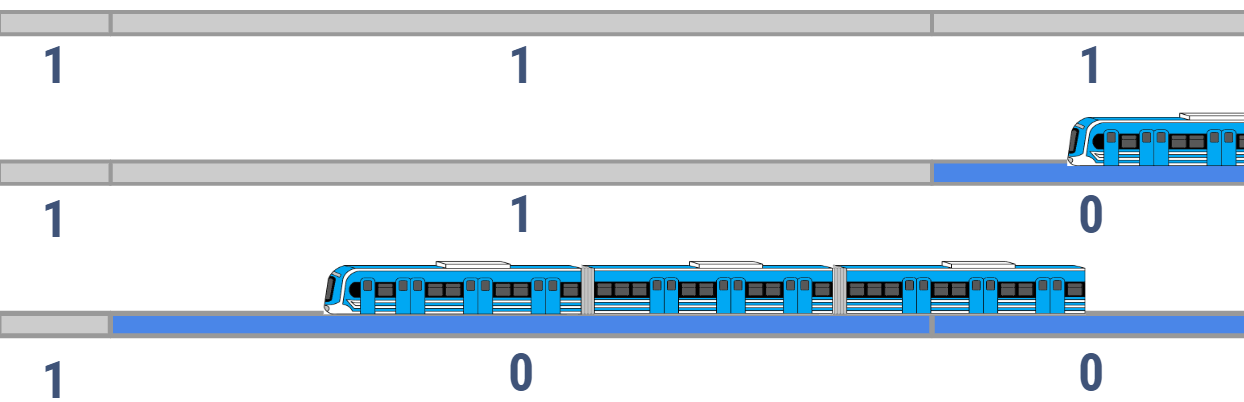
\includegraphics[width=1\textwidth]{Figuras/circuito_via}
        \centering\caption{Circuito de vía libre y ocupado.}
        \label{fig:deteccion_1}
    \end{figure}

En caso de que la alimentación se interrumpa, el cableado sufra alguna falla, vandalismo, inundación, o que efectivamente una formación ocupe la sección, el circuito de vía reportará que la sección se encuentra ocupada. De esta manera, solo es posible recibir un reporte de sección desocupada cuando la sección efectivamente se encuentre desocupada. A este principio se le denomina fail-safe [REF]. Es decir, si por alguna razón algo falla, el sistema adopta la condición más restrictiva, mitigando la posibilidad de una situación peligrosa

Los sistemas contadores de ejes (Figura \ref{fig:deteccion_2}) consisten en sensores pasivos instalados en la cara interna de unos de los rieles y un sistema externo de procesamiento de datos. Estos sistemas no dependen de la aplicación de tensiones en la vía. Además, no solo permiten detectar la presencia de una formación, sino que también pueden usarse para medir la integridad de la formación, sabiendo el largo esperado de la misma. 

    \begin{figure}[!h]
        \centering
        \includegraphics[width=1\textwidth]{example-image}
        \centering\caption{Contadores de ejes.}
        \label{fig:deteccion_2}
    \end{figure}

Al igual que los circuitos de vía, los sistemas contadores de eje siguen el principio de fail-safe, adoptando la condición mas restrictiva en caso de falla. Ambos sistemas pueden utilizarse en simultáneo, de ser requerido.
\subsubsection{Estaciones ferroviarias}

Las estaciones ferroviarias son las zonas donde las formaciones pueden detenerse para que los pasajeros puedan descender y nuevos pasajeros puedan abordar. En función del tamaño de las formaciones y la geografía del lugar, las plataformas desde donde ascienden y descienden los pasajeros pueden estar elevadas con respecto al suelo o a ras del mismo. El largo de las plataformas también depende de la cantidad de coches de las formaciones.

Como puede verse en la Figura \ref{fig:estacion_1}, las estaciones ferroviarias incluyen no solo a las plataformas, sino que también pueden centralizar el control de varias operaciones logísticas como la asignación de rutas. No obstante, en este trabajo nos referiremos a las estaciones como plataformas indistintamente.

    \begin{figure}[!h]
        \centering
        \includegraphics[width=1\textwidth]{example-image}
        \centering\caption{XXXXX.}
        \label{fig:estacion_1}
    \end{figure}

Las estaciones de mayor complejidad o de mayor convergencia de ramales suelen concentrar el control de la estación donde se encuentran y varias estaciones vecinas. Las estaciones terminales, a menudo, pueden incluso tener control total de varios ramales completos.
\subsubsection{Cruces ferroviarios}

Los cruces ferroviarios son la intersección entre la vía ferroviaria y una ruta vehicular o peatonal. Estos cruces pueden ser bajo nivel (túnel por debajo de la vía), sobre nivel (puente vehicular por sobre la vía) o a nivel. Un paso a nivel es una zona muy crítica del sistema ferroviario, ya que, a diferencia de un paso sobre nivel o bajo nivel, conviven simultáneamente la formación y el transito vehicular y peatonal. En la Figura \ref{fig:cruce_1} se ilustra la intersección entre el tendido ferroviario, un cruce vehicular y un cruce peatonal.

    \begin{figure}[!h]
        \centering
        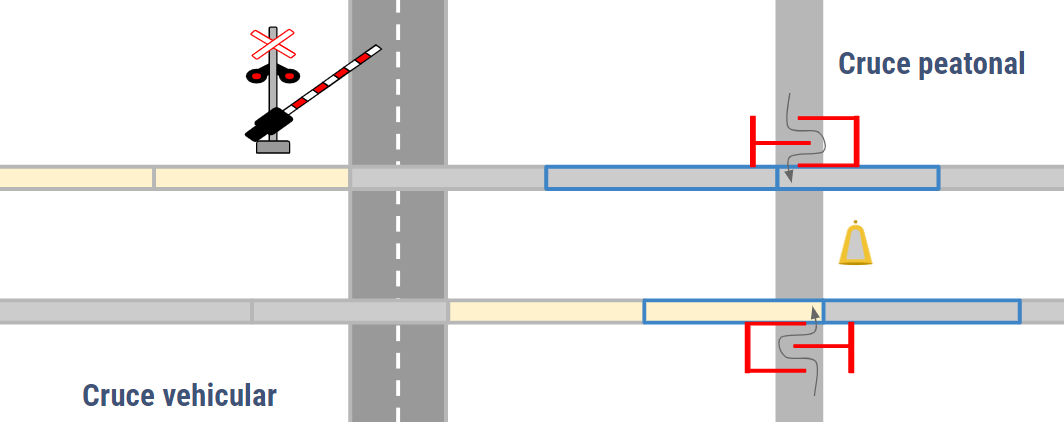
\includegraphics[width=1\textwidth]{Figuras/cruce}
        \centering\caption{XXXXX.}
        \label{fig:cruce_1}
    \end{figure}
    
Los pasos a nivel peatonales incluyen un pequeño laberinto zigzagueante para forzar al peatón a aminorar su marcha y ver a ambos lados antes de cruzar las vías. A menudo suelen estar acompañados de indicaciones lumínicas y sonoras que se accionan tan pronto el tren se encuentre dentro de un rango de varios metros cercano al paso a nivel.

Los pasos a nivel vehiculares añaden barreras ferroviarias para detener el tráfico vehicular cuando un tren se encuentra dentro de un rango de seguridad definido.  El sistema de control de la barrera mantiene el brazo de esta en alto para permitir la circulación vehicular. Si un tren es detectado cerca del paso a nivel, se desenergiza la barrera y comienza a descender el brazo por efecto de la gravedad. Solo cuando la barrera baja, el tren tiene permitido avanzar sobre el cruce, siendo el paso a nivel un sector de altísimo riesgo. Al desocuparse las secciones próximas al paso a nivel, la barrera vuelve a energizarse y se sitúa en estado alto nuevamente, a la espera de otro tren para reiniciar el proceso. 

Se debe destacar que el mismo proceso de descenso de la barrera ocurrirá si esta se desenergiza por una falla electricomecánica y/o pérdida de alimentación. Es decir, el sistema asumirá el estado más seguro ante cualquiera de los mencionados fallos, siguiendo el principio de falla segura.
\subsubsection{Máquina de cambios}

    \lipsum[1]

    \begin{figure}[h]
        \centering
        \includegraphics[width=0.5\textwidth]{example-image}
        \centering\caption{XXXXX.}
        \label{fig:cambios_1}
    \end{figure}

    \lipsum[1]
\subsubsection{Señales ferroviarias}

\lipsum[1]

\lipsum[1]
\includegraphics{example-image}
\lipsum[1]
